\documentclass{beamer}

\usepackage[utf8]{inputenc}
\usepackage{default}
\usepackage{tikz}
\usepackage{environ}
\usepackage{lipsum}
\usepackage{amssymb}
\usetikzlibrary{patterns,decorations.markings}

\newcommand{\halfmargin}{0.05\paperwidth}
\newcommand{\margin}{0.10\paperwidth}

\newlength\mywd
\setlength\mywd{.3\paperwidth}
\newlength\halfwd
\setlength\halfwd{.15\paperwidth}

\beamersetrightmargin{\margin}
\beamersetleftmargin{\margin}

\newlength\mysidebarcontentwidth
\setlength\mysidebarcontentwidth{.28\paperwidth}
\usetheme[width=\mywd]{myTheme}

\newif\ifUsedMaxNProc      \newif\ifUsedDimsNotDistrib    \newif\ifUsedDimsContig
\newif\ifUsedMinMPI        \newif\ifUsedMinMemory         \newif\ifUsedNoMemAlloc
\newif\ifUsedMinCopy

\UsedMaxNProcfalse         \UsedDimsNotDistribfalse       \UsedDimsContigfalse
\UsedMinMPIfalse           \UsedMinMemoryfalse            \UsedNoMemAllocfalse
\UsedMinCopyfalse

\newif\ifTargetMaxNProc    \newif\ifTargetDimsNotDistrib  \newif\ifTargetDimsContig
\newif\ifTargetMinMPI      \newif\ifTargetMinMemory       \newif\ifTargetNoMemAlloc
\newif\ifTargetMinCopy

\TargetMaxNProcfalse       \TargetDimsNotDistribfalse     \TargetDimsContigfalse
\TargetMinMPIfalse         \TargetMinMemoryfalse          \TargetNoMemAllocfalse
\TargetMinCopyfalse
 
\usepackage{pifont}
\newcommand{\cmark}{\ding{51}}%
\newcommand{\done}{\raisebox{-.5em}{\rlap{\large$\square$}{\raisebox{2pt}{\hspace{2pt}\cmark}}%
\hspace{2.5pt}}}

\newenvironment{todolist}
 {
  \begin{list}{\raisebox{-.5em}{\large$\square$}}
   { \setlength{\itemsep}{1em}      \setlength{\parsep}{0pt}
     \setlength{\topsep}{0pt}       \setlength{\partopsep}{0pt}
     \setlength{\leftmargin}{3.5em} \setlength{\labelwidth}{3.5em}
     \setlength{\labelsep}{1em}     
   }
 }
 {
  \end{list}
 }

\makeatletter
\setbeamertemplate{sidebar left}{%
  \vspace*{\fill}
  \begin{minipage}{\mysidebarcontentwidth}
  \tiny
  \color{white}
   \begin{todolist}
    \ifUsedDimsNotDistrib \item[\done] \else \item \fi
    { \ifTargetDimsNotDistrib \bf \fi The dimensions used by the operator are not distributed}
    
    \ifUsedDimsContig \item[\done] \else \item \fi
    {\ifTargetDimsContig \bf \fi  The dimensions used by the operator are contiguous}
    
    \ifUsedMaxNProc \item[\done] \else \item \fi
    { \ifTargetMaxNProc \bf \fi The number of processes that can be used is maximised}
    
    \ifUsedMinMPI \item[\done] \else \item \fi
    { \ifTargetMinMPI \bf \fi  The number of MPI messages sent and received is minimised}
    
    \ifUsedMinMemory \item[\done] \else \item \fi
    { \ifTargetMinMemory \bf \fi  The memory required is minimised}
    
    \ifUsedNoMemAlloc \item[\done] \else \item \fi
    { \ifTargetNoMemAlloc \bf \fi  After setup no memory is allocated}
    
    \ifUsedMinCopy \item[\done] \else \item \fi
    { \ifTargetMinCopy \bf \fi  As little copying of data as possible is used}
   \end{todolist}
  \end{minipage}\par
  \vfill
  \parbox{\mywd}{\centering\textcolor{white}{\insertauthor}}
  \vspace*{0.6cm}
}
\setlength\beamer@sidebarwidth{\mywd}

\makeatother

\NewEnviron{NoSidebarFrame}[1][]{%
\begin{frame}[plain]{#1}
\hspace*{-\mywd}
\begin{minipage}{\dimexpr\paperwidth-\halfmargin-\halfmargin\relax}
\centering
\BODY
\end{minipage}
\end{frame}
}

\definecolor{contigColor}{RGB}{170, 255, 184}

% -------------------------------------------------------------------------------------------------------------------------------
% -------------------------------------------------------------------------------------------------------------------------------
% -------------------------------------------------------- DOCUMENT -------------------------------------------------------------
% -------------------------------------------------------------------------------------------------------------------------------
% -------------------------------------------------------------------------------------------------------------------------------


\begin{document}

\begin{NoSidebarFrame}[Coordinate system]
 \only<1>{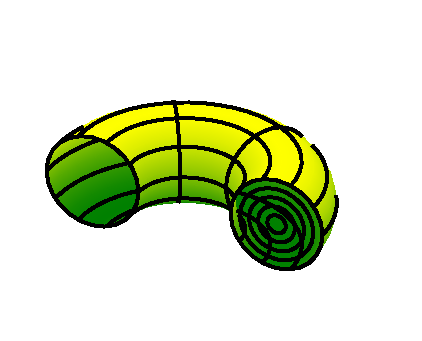
\includegraphics[width=0.8\textwidth]{Tokamak/Tokamak}}
 \only<2>{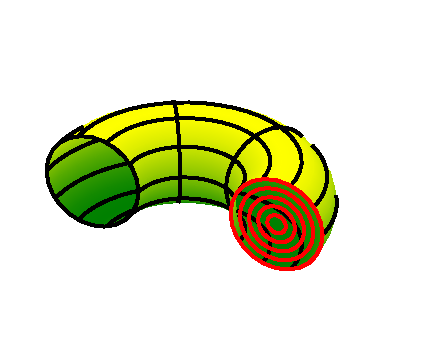
\includegraphics[width=0.8\textwidth]{Tokamak/TokamakRCoords}}
 \only<3>{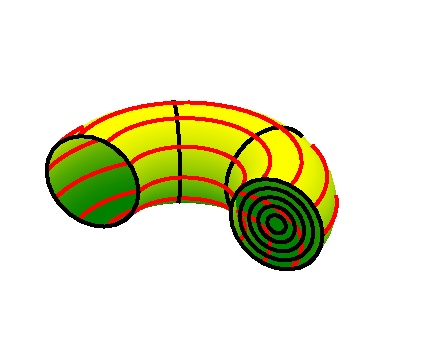
\includegraphics[width=0.8\textwidth]{Tokamak/TokamakQCoords}}
 \only<4>{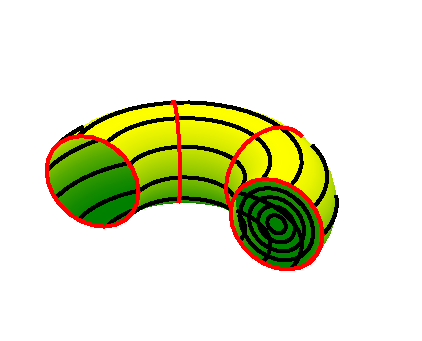
\includegraphics[width=0.8\textwidth]{Tokamak/TokamakZCoords}}
\end{NoSidebarFrame}

\begin{NoSidebarFrame}[Parallelisation Conditions]
 \begin{enumerate}
 \item The number of processes that can be used is maximised \label{Condition Max nprocs}
 \item The dimensions used by the operator are not distributed  \label{Condition distribution}
 \item The dimensions used by the operator are contiguous \label{Condition contiguous}
 \item The number of MPI messages sent and received is minimised \label{Condition MPI overhead}
 \item The memory required is minimised \label{Condition memory}
 \item After setup no memory is allocated \label{Condition allocation}
 \item As little copying of data as possible is used \label{Condition copying}
\end{enumerate}
\end{NoSidebarFrame}

\TargetDimsNotDistribtrue

\begin{frame}{Advection Operators}
\begin{overlayarea}{\textwidth}{10cm}
 \begin{equation}
  \partial_t f + v_\parallel \nabla_\parallel f = 0 \label{eq::Advection1}
 \end{equation}
 
 \only<1> {
 
 \begin{center}
  ($r$,\colorbox{white}{\strut $\theta$},\colorbox{white}{\strut $z$},$v_\parallel$)
 \end{center}
 }
 \only<2->{
 \begin{center}
  ($r$,\colorbox{contigColor}{\strut $\theta$},\colorbox{contigColor}{\strut $z$},$v_\parallel$)
 \end{center}}
 
 \only<3->{
 \begin{equation}
  \partial_t f + \nabla_\parallel \tilde{\phi} \partial_{v_{\parallel}} f = 0 \label<3->{eq::Advection2}
 \end{equation}
 }
 
 \only<3>{
 \begin{center}
  ($r$,$\theta$,$z$,\colorbox{white}{\strut $v_\parallel$})
 \end{center}
 }
 \only<4->{
 \begin{center}
  ($r$,$\theta$,$z$,\colorbox{contigColor}{\strut $v_\parallel$})
 \end{center}
 }
 
 \only<5->{
 \begin{equation}
  \partial_t f + \{\tilde{\phi}, f\} = 0 \label<5->{eq::Advection3}
 \end{equation}}
 
 \only<5>{
 \begin{center}
  (\colorbox{white}{\strut $r$},\colorbox{white}{\strut $\theta$},$z$,$v_\parallel$)
 \end{center}}
 \only<6->{
 \begin{center}
  (\colorbox{contigColor}{\strut $r$},\colorbox{contigColor}{\strut $\theta$},$z$,$v_\parallel$)
 \end{center}}
 
 \end{overlayarea}
\end{frame}

\TargetDimsNotDistribfalse
\UsedDimsNotDistribtrue
\TargetDimsContigtrue

\begin{frame}{Advection Operators}
\begin{overlayarea}{\textwidth}{10cm}
\only<1>{
  \[
   \partial_t f + v_\parallel \nabla_\parallel f = 0 \tag{\ref{eq::Advection1}}
  \]
 
 \begin{center}
  ($r$,\colorbox{contigColor}{\strut $\theta$},\colorbox{contigColor}{\strut $z$},$v_\parallel$)
 \end{center}
 
 \[
  \partial_t f + \nabla_\parallel \tilde{\phi} \partial_{v_{\parallel}} f = 0 \tag{\ref{eq::Advection2}}
 \]
 
 \begin{center}
  ($r$,$\theta$,$z$,\colorbox{contigColor}{\strut $v_\parallel$})
 \end{center}
 
 \[
  \partial_t f + \{\tilde{\phi}, f\} = 0 \tag{\ref{eq::Advection3}}
 \]
 
 \begin{center}
  (\colorbox{contigColor}{\strut $r$},\colorbox{contigColor}{\strut $\theta$},$z$,$v_\parallel$)
 \end{center}}
 \only<2->{
 \[
  \partial_t f + v_\parallel \nabla_\parallel f = 0 \tag{\ref{eq::Advection1}}
 \]
 
 \begin{center}
  ($r$,\strut $v_\parallel$,\colorbox{contigColor}{\strut $\theta$},\colorbox{contigColor}{\strut $z$})
 \end{center}
 
 \[
  \partial_t f + \nabla_\parallel \tilde{\phi} \partial_{v_{\parallel}} f = 0 \tag{\ref{eq::Advection2}}
 \]
 
 \begin{center}
  ($r$,$\theta$,$z$,\colorbox{contigColor}{\strut $v_\parallel$})
 \end{center}
 
 \[
  \partial_t f + \{\tilde{\phi}, f\} = 0 \tag{\ref{eq::Advection3}}
 \]
 
 \begin{center}
  ($z$,$v_\parallel$,\colorbox{contigColor}{\strut $r$},\colorbox{contigColor}{\strut $\theta$})
 \end{center}
 }
 
 \end{overlayarea}
\end{frame}

\TargetDimsContigfalse
\UsedDimsContigtrue
\TargetMaxNProctrue

\begin{frame}{Dimension Ordering}
 \begin{minipage}{.3\textwidth}
 \centering
  ($r$,\strut $v_\parallel$,\colorbox{contigColor}{\strut $\theta$},\colorbox{contigColor}{\strut $z$})
 \end{minipage}
 \begin{minipage}{.3\textwidth}
 \centering
  ($r$,$\theta$,$z$,\colorbox{contigColor}{\strut $v_\parallel$})
 \end{minipage}
 \begin{minipage}{.3\textwidth}
 \centering
  ($z$,$v_\parallel$,\colorbox{contigColor}{\strut $r$},\colorbox{contigColor}{\strut $\theta$})
 \end{minipage}
 \vspace{1.5em}
 
 \only<1>{
 \begin{minipage}{.3\textwidth}
 \centering
  $n_r\cdot n_{v_\parallel}$
 \end{minipage}
 \begin{minipage}{.3\textwidth}
 \centering
  $n_r\cdot n_{\theta}\cdot n_z$
 \end{minipage}
 \begin{minipage}{.3\textwidth}
 \centering
 \tikz \node[draw,circle,inner sep=1pt,draw=white] {$n_z\cdot n_{v_\parallel}$};
 \end{minipage}
 }
 \only<2->{
 \begin{minipage}{.3\textwidth}
 \centering
  $n_r\cdot n_{v_\parallel}$
 \end{minipage}
 \begin{minipage}{.3\textwidth}
 \centering
  $n_r\cdot n_{\theta}\cdot n_z$
 \end{minipage}
 \begin{minipage}{.3\textwidth}
 \centering
 \tikz \node[draw,circle,inner sep=1pt] {$n_z\cdot n_{v_\parallel}$};
 \end{minipage}
 }
 
 \vspace{1em}
 
 \centering
 
 \begin{itemize}
  \item<2-> Flux-aligned method allows fewer points to be used along z
  \item<3-> A fine grid is required in the poloidal plane
 \end{itemize}

\end{frame}


\begin{frame}
 \begin{minipage}[b]{.45\textwidth}
  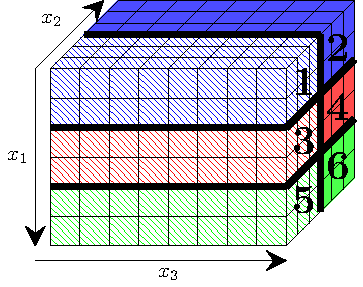
\includegraphics[width=\textwidth]{Probleme/Start}
 \end{minipage}
 \hspace{.05\textwidth}
 \begin{minipage}[b]{.45\textwidth}
  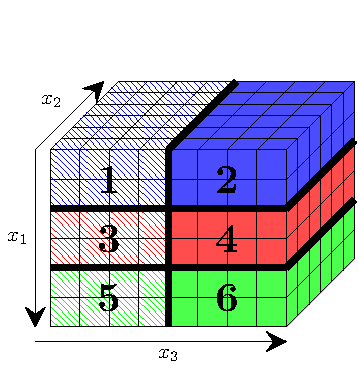
\includegraphics[width=\textwidth]{Probleme/End}
 \end{minipage}
 
 \begin{minipage}{.45\textwidth}
 \centering
 \Large
  $(x_1,x_2,x_3)$
 \end{minipage}
 \hspace{.05\textwidth}
 \begin{minipage}{.45\textwidth}
 \centering
 \Large
  $(x_1,x_3,x_2)$
 \end{minipage}

\end{frame}

 \UsedMaxNProctrue
 
 
\begin{frame} 
 \begin{minipage}[b]{.4\textwidth}
  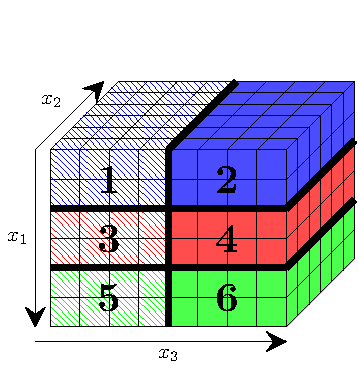
\includegraphics[scale=0.6]{Probleme/End}
 \end{minipage}
 \hspace{.05\textwidth}
 \begin{minipage}[b]{.45\textwidth}
  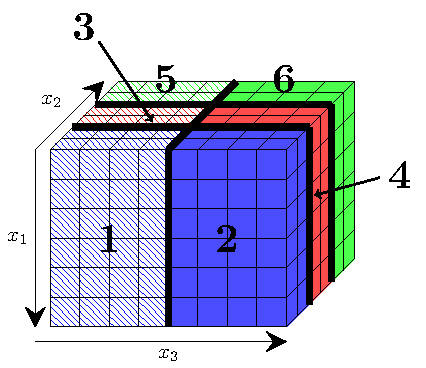
\includegraphics[scale=0.6]{Probleme/End2}
 \end{minipage}
 
 \begin{minipage}{.45\textwidth}
 \centering
 \Large
  $(x_1,x_3,x_2)$
 \end{minipage}
 \hspace{.05\textwidth}
 \begin{minipage}{.45\textwidth}
 \centering
 \Large
  $(x_2,x_3,x_1)$
 \end{minipage}
\end{frame}


\end{document}
